% Every frame has presenter notes. Source labels refer to the dissertation,
% not to labels in this standalone presentation. A = unscaled first difference;
% B = flow data coefficient (renamed from A_data to prevent a notation collision).

\section{The inverse problems}
\begin{frame}[plain]
\titlepage
\talknote{Opening; about 30 seconds.}{The motivating question is how to estimate images, motion, and depth when the sensor reports changes rather than conventional image frames. The mathematical thread is the interaction of observation null spaces, regularization, and identifiability.}{The talk first introduces the sensor without assuming a computer-vision background, then develops the three inverse problems. The defense date is intentionally not specified beyond the semester.}
\end{frame}

\begin{frame}{Scenes recovered from brightness changes}
\centering
\begin{columns}[T]
\column{.32\textwidth}\centering
\vspace{1mm}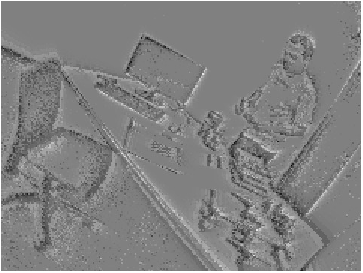
\includegraphics[width=\linewidth,height=3.6cm,keepaspectratio]{figures/office/office_ex_11.pdf}\par\vspace{.6mm}
% source: Ch. 2 subsubsec:datasets and subsec:validation_office; approx. 2.5M events.
{\footnotesize\textbf{Office}, handheld; $\approx2.5$M events}
\column{.32\textwidth}\centering
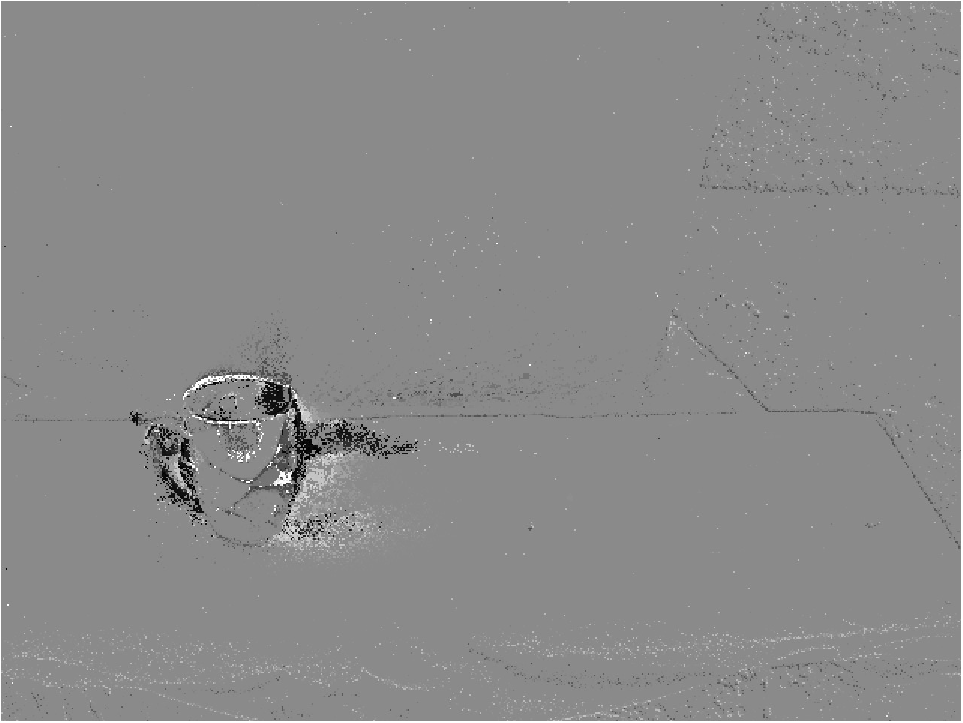
\includegraphics[width=\linewidth,height=1.85cm,keepaspectratio]{figures/cup/cup_ex_5.pdf}\par\vspace{.6mm}
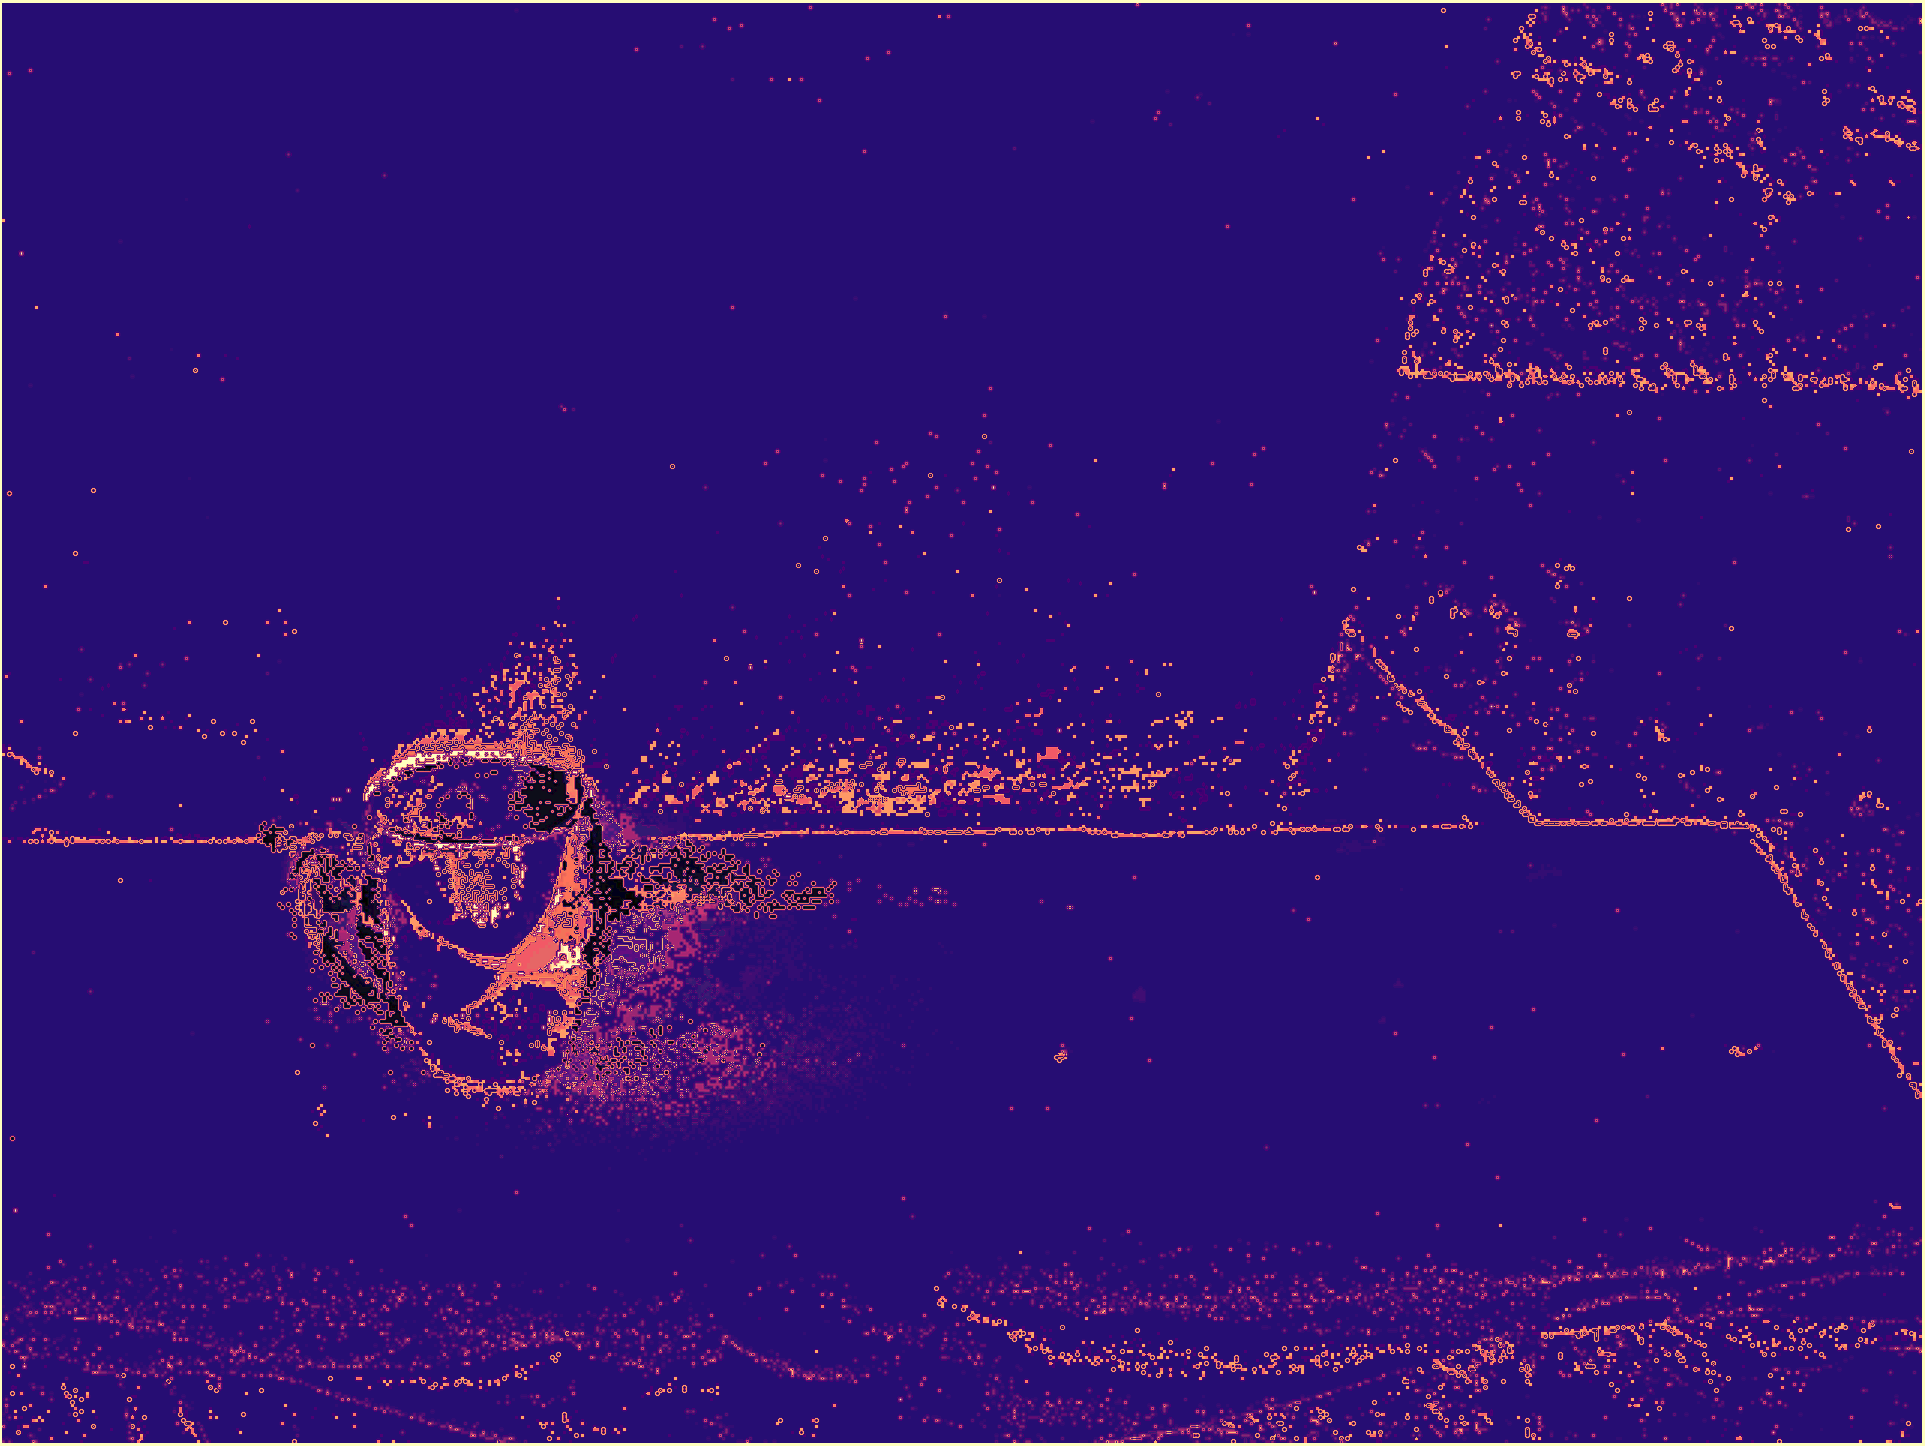
\includegraphics[width=\linewidth,height=1.85cm,keepaspectratio]{figures/cup/cm_cup/cup_5_0.0510_colormapped.png}\par
% source: Ch. 2 subsubsec:datasets and f:cup; approx. 350,000 events.
{\footnotesize\textbf{Bullet hits a cup}; $\approx350$K events}
\column{.32\textwidth}\centering
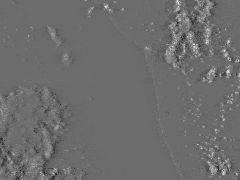
\includegraphics[width=\linewidth,height=1.85cm,keepaspectratio]{figures/ISS/110_0993g_reflected.png}\par\vspace{.6mm}
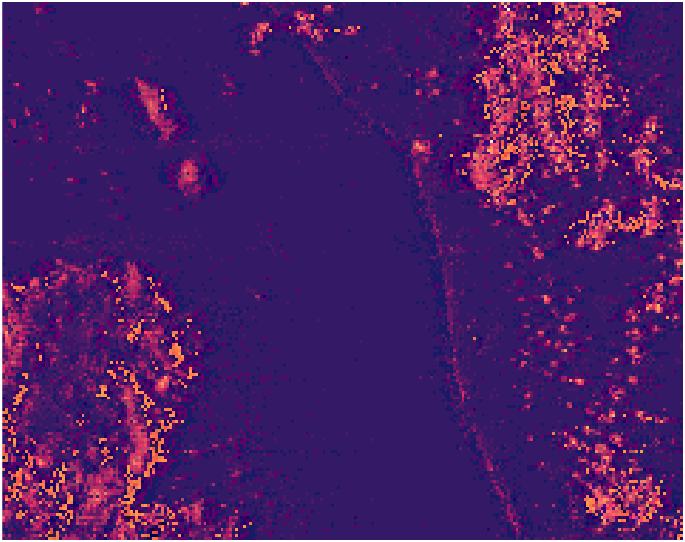
\includegraphics[width=\linewidth,height=1.85cm,keepaspectratio]{figures/ISS/110_0993_reflected.png}\par
% source: Ch. 2 subsubsec:datasets and f:iss; approx. 2 million events.
{\footnotesize\textbf{ISS} (Falcon Neuro); $\approx2$M events}
\end{columns}
{\scriptsize\color{muted}Cup and ISS: grayscale (top) and false color (bottom) of the same reconstructed frame.\par}
\vspace{1mm}\raggedright\small
% source: Gallego et al., "Event-based Vision: A Survey," IEEE TPAMI 44(1), 2022, abstract: microsecond temporal resolution, low power consumption.
Each pixel reports when its brightness changes, with microsecond timing and low power~\cite{gallego2022event}.\par\smallskip
This dissertation recovers images, motion, and depth from these changes, with guarantees on the estimates and computation simple enough for on-board use.
% source detail: Ch. 2, subsec:validation, f:office, f:cup, f:iss; datasets in subsubsec:datasets.
\src{\dref{Figure}{f:office}, \dref{Figure}{f:cup}, and \dref{Figure}{f:iss}; \dref{Section}{subsec:validation}. Data: office~\cite{gallego2017accurate}, cup~\cite{rebecq2021highspeed}, Falcon Neuro~\cite{mcharg2022falcon}.}
\talknote{Motivation; about 2 minutes. Show the results before any mathematics.}{Office: a handheld camera in an office; the desk objects and the person are recognizable. Cup: a bullet strikes a ceramic cup from the left; the event stream resolves the fracture and spray, which a standard-rate frame camera would blur. ISS: the Falcon Neuro event cameras on the International Space Station viewing the eastern coastline of Honduras; land--water boundaries and clouds are visible although the scene changes slowly and the events are sparse. All three come from events alone, with one per-pixel solve and no intensity frames.}{Why it matters: fast scenes, wide brightness ranges, and platforms with tight power budgets such as drones and spacecraft. On those platforms the estimator must also be cheap and predictable, which the reconstruction chapter quantifies. Grayscale and false color are display choices, not calibrated brightness. Transition: what the sensor reports, and why that makes these problems mathematically interesting.}
\end{frame}

\begin{frame}{Why an event camera? Each pixel reports its own changes}
\begin{columns}[T]
\column{.48\textwidth}
\centering\textbf{Conventional camera}\par\smallskip
\begin{tikzpicture}[x=.62cm,y=.23cm,>=Latex]
\draw[->,muted] (0,0)--(8.4,0) node[right,font=\scriptsize] {$t$};
\draw[->,muted] (0,0)--(0,6.8) node[above,font=\scriptsize] {pixel};
\foreach \t in {1,3,5,7}{\foreach \r in {1,...,6}{\fill[muted!45] (\t-.18,\r-.32) rectangle (\t+.18,\r+.32);}}
\draw[amber,dashed,thick] (.6,.6)--(7.4,6.4);
\node[font=\scriptsize,align=center] at (4,-1.3) {every pixel, at fixed frame times};
\end{tikzpicture}
\column{.48\textwidth}
\centering\textbf{Event camera}\par\smallskip
\begin{tikzpicture}[x=.62cm,y=.23cm,>=Latex]
\draw[->,muted] (0,0)--(8.4,0) node[right,font=\scriptsize] {$t$};
\draw[->,muted] (0,0)--(0,6.8) node[above,font=\scriptsize] {pixel};
\draw[amber,dashed,thick] (.6,.6)--(7.4,6.4);
\foreach \r in {1,...,6}{\fill[teal] ({.6+(\r-.6)*6.8/5.8},\r) circle (2.6pt);\fill[amber] ({.6+(\r-.6)*6.8/5.8+.9},\r) circle (2.6pt);}
\node[font=\scriptsize,align=center] at (4,-1.3) {only where and when brightness changes};
\end{tikzpicture}
\end{columns}
\vspace{-1mm}
{\footnotesize Dashed line: the leading edge of a moving bright bar. Teal: brightening ($+$); amber: darkening ($-$).}
\begin{itemize}\footnotesize
% source: Gallego et al., "Event-based Vision: A Survey," IEEE TPAMI 44(1), 2022, abstract (gmuETD.bib gallego2022event).
\item Microsecond timestamps, about $140$\,dB dynamic range versus $60$\,dB, low power, little motion blur~\cite{gallego2022event}.
\end{itemize}
% source detail: Ch. 1; Ch. 2, Neuromorphic Cameras overview. Diagram is schematic.
\src{\dref{Chapter}{ch:monocular_reconstruction}, neuromorphic camera overview; Gallego et al.~\cite{gallego2022event}. Diagram is schematic.}
\talknote{Accessibility primer; about two minutes. Assume no event-camera background.}{Point to the left panel: a conventional camera samples every pixel at the same frame times, whether or not anything changes, and averages over its exposure. Point to the right panel: the same moving bright bar produces a brightening event when its leading edge reaches a pixel and a darkening event when its trailing edge leaves. This is why event displays often look like moving outlines: a boundary passing across a pixel changes its brightness, while a uniform region undergoing the same translation produces little activity. The sensor responds to temporal brightness change; illumination changes can also trigger events. The survey figures quoted on the slide are the standard sensor-class numbers from Gallego et al.\ (TPAMI 2022), not measurements made in this dissertation.}{Give the committee the one idea the whole talk uses: events record when the log-brightness at a pixel changed by a fixed amount, so the data determine changes and leave the starting brightness free. Then turn to the next slide for the exact threshold rule. If asked about hardware: the dissertation's MVSEC, office, and cup data come from DAVIS346 sensors, and the orbital data from the Falcon Neuro instrument on the ISS.}
\end{frame}

\begin{frame}{An event camera: each pixel reports threshold crossings}
\begin{columns}[c]
\column{.57\textwidth}
\begin{tikzpicture}[x=.72cm,y=.72cm,>=Latex]
\draw[->,muted] (0,0)--(7,0) node[right] {$t$};
\draw[->,muted] (0,0)--(0,4) node[above] {$L=\log I$};
\draw[teal,very thick] (0,1)--(1,1.2)--(2,2)--(3,3)--(4,3.15)--(5,2)--(6,1)--(6.6,1.2);
\draw[amber,dashed] (0,1)--(2,1)--(2,2)--(3,2)--(3,3)--(5,3)--(5,2)--(6,2)--(6,1)--(6.6,1);
\foreach \x/\y in {2/2,3/3,5/2,6/1}{\fill[ink] (\x,\y) circle (2pt);\draw[muted,dotted] (\x,\y)--(\x,-.55);}
\node[teal] at (2,-.85) {$+$};\node[teal] at (3,-.85) {$+$};
\node[amber] at (5,-.85) {$-$};\node[amber] at (6,-.85) {$-$};
\node[muted,align=left,font=\scriptsize] at (3.4,3.8) {Solid: log-intensity\\ Dashed: reset reference};
\end{tikzpicture}
\column{.40\textwidth}
An event is a tuple
\[e_k=(\mathbf x_k,s_k,p_k),\qquad p_k=\pm1.\]
For the ideal threshold model,
\[L(\mathbf x_k,s_k)-L(\mathbf x_k,s_k^-)=p_k c_{\rm th}.\]
The preceding reset $s_k^-$ is \textbf{local to that pixel}.
\end{columns}
% source detail: Ch. 2, eq:polarity; Ch. 3, eq:event\_integral. Diagram is schematic.
\src{\dref{Eq.}{eq:polarity}; \dref{Eq.}{eq:event_integral}; ideal threshold model~\cite{lichtsteiner2008128}. Diagram is schematic.}
\talknote{Sensor primer; 90 seconds.}{Follow the solid curve. A positive event is emitted after an upward change of one threshold from the most recent reset; a negative event follows a downward change. Different pixels have independent reset times, so the observation times are asynchronous. Neuromorphic here refers to the change-triggered sensing architecture; these estimators do not require a neural network.}{The equality is an ideal noiseless threshold model. Real threshold uncertainty, missed events, refractory effects, and overshoot create discrepancies. The diagram is conceptual, with arbitrary axes and no claim about measured latency. A stationary bright pixel can produce no events: zero activity is not zero intensity.}
\end{frame}

\begin{frame}{From events to images, motion, and depth}
\begin{columns}[T]
\column{.32\textwidth}
\centering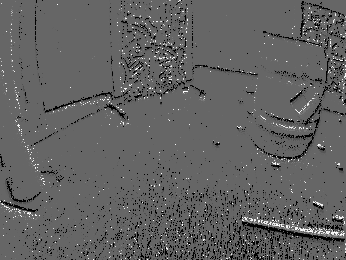
\includegraphics[width=\linewidth,height=2.1cm,keepaspectratio]{figures/indoor_flying2_t47p6/bspline_reconstruction.png}\par\vspace{1mm}
{\small\textbf{Image reconstruction}}\par
{\footnotesize Ch.\ 2}\par
{\scriptsize Grayscale: reconstructed value.}
\column{.32\textwidth}
\centering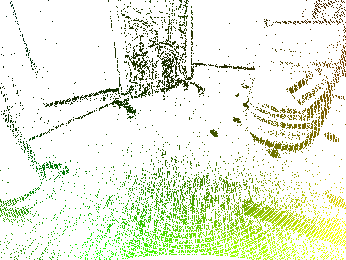
\includegraphics[width=\linewidth,height=2.1cm,keepaspectratio]{figures/indoor_flying2_t47p6/cmax_flow_event_pixels.png}\par\vspace{1mm}
{\small\textbf{Optical-flow estimate}}\par
{\footnotesize Ch.\ 3; event-active pixels}\par
\begin{tikzpicture}[baseline=(wheel.center)]
\node[inner sep=0pt] (wheel) at (0,0) {\phantom{\rule{.7cm}{.7cm}}};
\foreach \a in {0,10,...,350}{%
  \pgfmathsetmacro{\hue}{\a/360}\definecolor{wheelhue}{hsb}{\hue,1,1}%
  \begin{scope}\clip (0,0)--(-\a:.32)--(-\a-11:.32)--cycle;
  \shade[inner color=black,outer color=wheelhue] (0,0) circle (.32);\end{scope}}
\node[font=\tiny,inner sep=1pt] at (0:.47) {$\rightarrow$};\node[font=\tiny,inner sep=1pt] at (-90:.46) {$\downarrow$};
\node[font=\tiny,inner sep=1pt] at (180:.47) {$\leftarrow$};\node[font=\tiny,inner sep=1pt] at (90:.46) {$\uparrow$};
\node[font=\tiny,align=left,anchor=west] at (.62,0) {hue: direction\\brightness: size\\(full at $\approx14$\,px)};
\end{tikzpicture}
\column{.32\textwidth}
\centering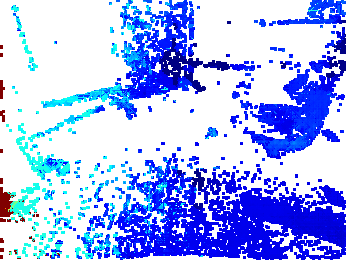
\includegraphics[width=\linewidth,height=2.1cm,keepaspectratio]{figures/indoor_flying2_t47p6/wls_depth.png}\par\vspace{1mm}
{\small\textbf{Stereo-depth estimate}}\par
{\footnotesize Ch.\ 4}\par
% source: figures/indoor_flying2_t47p6/metadata.json, wls_display.
\begin{tikzpicture}
\foreach \i in {0,...,59}{\pgfmathsetmacro{\t}{\i/59}%
  \pgfmathsetmacro{\jr}{min(max(1.5-abs(4*\t-3),0),1)}\pgfmathsetmacro{\jg}{min(max(1.5-abs(4*\t-2),0),1)}\pgfmathsetmacro{\jb}{min(max(1.5-abs(4*\t-1),0),1)}%
  \definecolor{jetstep}{rgb}{\jr,\jg,\jb}\fill[jetstep] ({.04*\i},0) rectangle ({.04*\i+.05},.16);}
\node[font=\tiny,anchor=north] at (0,0) {$0.5$};\node[font=\tiny,anchor=north] at (2.4,0) {$8$\,m};
\node[font=\tiny,anchor=south] at (1.2,.16) {depth (jet), near to far};
\end{tikzpicture}
\end{columns}
\vspace{1mm}
% source: figures/indoor_flying2_t47p6/metadata.json, reconstruction and flow timestamps and WLS center.
{\footnotesize MVSEC~\cite{MVSEC2018} indoor\_flying2, drone-mounted event cameras, near $47.6$\,s; stereo depth uses both.}
% source detail: Saved HPC estimates; provenance, hashes, timestamps, display scales, and masks in figures/indoor_flying2_t47p6/metadata.json.
\src{Methods: \dref{Chapter}{ch:monocular_reconstruction}, \dref{Chapter}{ch:optical_flow}, and \dref{Chapter}{ch:stereo_depth_estimation}; MVSEC~\cite{MVSEC2018}.}
% source: figures/indoor_flying2_t47p6/metadata.json, timestamps, observation windows, display rules, and geometry.
\talknote{Accessibility primer; 90 seconds. Introduce the three estimated outputs.}{Left: temporal image reconstruction. Middle: optical-flow estimate, with color encoding direction and displacement magnitude at pixels that recorded events. Right: stereo depth. All three show the same indoor flying 2 scene. Present the panels as the three estimation targets. Explain the brightness baseline, motion along an edge, and stereo correspondence.}{If asked which methods: B-spline kernel with sigmoid weights; contrast maximization, whose nonconvex objective lies outside the quadratic family analyzed later (existence result in backup); weighted least squares. Reconstruction: 47.690 s. Flow: 47.592--47.719 s; color magnitude represents displacement over this window. White flow pixels have zero events: the mask shows event support, not confidence. WLS: center 47.598 s, 250 ms window. Different windows and stereo rectification permit scene-level comparison, with separate pixel geometries. Depth colors clip to 0.5--8 m; white masks nonfinite values and the maximum finite depth. Reconstruction grayscale uses a histogram/percentile scale. Exact timestamps, normalization, and provenance are in the adjacent metadata file.}
\end{frame}

\begin{frame}{Three estimators, each well posed}
\renewcommand{\arraystretch}{1.6}
\begin{tabular}{>{\raggedright\arraybackslash}p{3.7cm}>{\raggedright\arraybackslash}p{9.7cm}}
\textbf{Reconstruction} (Ch.~2) & One tridiagonal solve per pixel; unique and stable for every positive weight.\\
\textbf{Optical flow} (Ch.~3) & Three event representations, one quadratic theory; unique flow when edges span two directions.\\
\textbf{Stereo depth} (Ch.~4) & A unique inner solve at each candidate depth; competitive MVSEC accuracy with the most scored points.\\
\end{tabular}\par
\vspace{5mm}
{\small The common question: which quantities do the events determine, and which does the model supply?\par}
% source detail: Chs. 1 and 5; Ch. 5, tab:contribution\_matrix; Ch. 2 thm:uniqueness; Ch. 3 thm:unified\_wellposedness; Ch. 4 thm:weighted\_spd and App. tab:unified\_benchmark (2.66M scored points, the largest).
\src{\dref{Table}{tab:contribution_matrix}; \dref{Theorem}{thm:uniqueness}, \dref{Theorem}{thm:unified_wellposedness}, \dref{Theorem}{thm:weighted_spd}.}
\talknote{What the talk shows; about 90 seconds.}{Reconstruction gets most of the time: the model, its uniqueness and stability, and its cost. Optical flow follows with the main theorem. Stereo is a one-slide summary. Each row names a result, not a topic.}{The common question links the rows: the events determine some quantities, and the model supplies the rest. The footer tracks the position along this route. Start with the sensor's observation model, which is where the reconstruction begins.}
\end{frame}

\section{Temporal reconstruction}
\begin{frame}{Start with one pixel: integrated changes on a temporal chain}
\begin{columns}[T]
\column{.54\textwidth}
Choose a unit-mass temporal kernel $\phi_{s_k}$:
\[e(t)=\sum_{k\text{ at this pixel}}p_k\phi_{s_k}(t).\]
\[y_i=\int_{t_i}^{t_{i+1}}e(t)\,dt.\]
The reconstruction times $t_i$ are chosen by the algorithm.
\column{.43\textwidth}
\[\A=\begin{pmatrix}-1&1&&\\&-1&1&\\&&\ddots&\ddots\end{pmatrix}.\]
\[\A\mathbf f\approx\mathbf y.\]
\[\ker\A=\operatorname{span}\{\mathbf1\}.\]
Events determine increments, leaving a constant free.
\end{columns}
\vspace{1mm}
{\footnotesize\textbf{In scene terms:} each pixel's log-brightness history is rebuilt on its own from how much it rose or fell in each interval. The model chooses the reference level; a pixel without events stays at that level, whatever its brightness.\par}
% source detail: Ch. 2, eq:exy, eq:Exy, eq:tempdiffA, lem:nullspace.
\src{\dref{Eq.}{eq:Exy}, \dref{Eq.}{eq:tempdiffA}, and \dref{Lemma}{lem:nullspace}.}
\talknote{Temporal observation model; 75 seconds.}{Suppress the pixel index to keep the notation readable. Integrating a unit-mass kernel across a bin assigns all or part of each event to that bin. Delta binning has no spread; Gaussian, rectangular, and spline kernels distribute influence over time. The entries of A are unscaled increments, not derivatives divided by a time step.}{If Af=0, every consecutive pair of components is equal, hence f is constant. Conversely A1=0. Under ideal threshold calibration the observed increments approximate changes in L/c\_th, with kernel-boundary, overshoot, and between-event endpoint errors. No absolute frame is used to set the baseline. Scene terms: each pixel's brightness history is rebuilt on its own; a pixel without events stays at the reference level.}
\end{frame}

\begin{frame}{Temporal kernels: how far each event's influence spreads}
\begin{columns}[c]
\column{.50\textwidth}
\begin{tikzpicture}
\begin{axis}[width=7.2cm,height=3.9cm,xmin=-.8,xmax=1.9,ymin=0,ymax=2.7,xtick={-.5,0,.5},xticklabels={$s-\frac w2$,$s$,$s+\frac w2$},ytick=\empty,xlabel={$t$},label style={font=\scriptsize},tick label style={font=\scriptsize},legend style={font=\tiny,at={(.99,.98)},anchor=north east,draw=none,fill=none}]
\addplot[muted,thick,const plot] coordinates {(-.8,0) (-.5,0) (-.5,1) (.5,1) (.5,0) (.9,0)};\addlegendentry{rectangular}
\addplot[amber,thick] coordinates {(-.8,0) (-.5,0) (0,2) (.5,0) (.9,0)};\addlegendentry{linear B-spline}
% source: analytic truncated Gaussian, sigma=w/6, Z=erf(3/sqrt 2)=0.9973 (Ch. 2 subsec:bumpsel).
\addplot[teal,thick,domain=-.5:.5,samples=80]{exp(-x^2/(2*(1/6)^2))/((1/6)*sqrt(2*pi)*0.9973)};\addlegendentry{Gaussian, $3\sigma=\frac w2$}
\draw[ink,very thick,-{Latex}] (axis cs:0,0)--(axis cs:0,2.6);
\end{axis}
\end{tikzpicture}
\par{\scriptsize Arrow: delta kernel (pure binning). Common support width $w$; schematic.}
\column{.47\textwidth}
\small Each kernel has unit mass, is a translate, and has compact support:
\[\int_{\R}\phi_s=1,\qquad \phi_s(t)=\phi_0(t-s).\]
Each event splits its sign $p_k$ across the bins it overlaps:
\[y_i=\sum_k p_k\int_{t_i}^{t_{i+1}}\phi_{s_k}(t)\,dt,\quad
\textstyle\sum_i y_i=\sum_k p_k\]
when every support lies inside $[t_0,t_N]$.
\end{columns}
% source detail: Ch. 2, subsec:bumpsel, prop:l1\_bump\_properties, prop:dist\_bump\_properties, tab:support\_widths.
\src{\dref{Proposition}{prop:l1_bump_properties}, \dref{Proposition}{prop:dist_bump_properties}; \dref{Table}{tab:support_widths}.}
\talknote{Kernel choice; 75 seconds.}{The four kernels are the ones evaluated in Chapter 2: delta (binning), truncated and renormalized Gaussian, B-spline, and rectangular. Unit mass means each event contributes exactly its sign in total; translation invariance means the bin integrals are a convolution; compact support means each event touches finitely many bins. The sum identity is exact: summing the bin integrals telescopes to the integral over the whole window, which is one when the event's full support lies in the window.}{The plotted widths are matched for display only; the evaluated parameters differ by kernel (Ch.\ 2 bump sweep). If asked which kernel is best: the indoor and outdoor rankings differ (discussion page on kernel performance), and the uniqueness theorem holds for every kernel because it depends only on $\A$ and positive weights. Transition: next, when these integrated observations approximate a physical brightness change.}
\end{frame}

\begin{frame}{From threshold crossings to an approximate observation}
\begin{columns}[c]
\column{.44\textwidth}
\begin{tikzpicture}[x=.71cm,y=.46cm,>=Latex]
\draw[->,muted] (0,0)--(7.3,0) node[right] {$t$};
\draw[->,muted] (0,0)--(0,3.9) node[above] {$L/c_{\rm th}$};
\draw[teal,very thick] (0,1)--(1,1.25)--(2,2)--(3,3)--(4,3.2)--(5,2)--(5.8,1.45)--(6.6,1.6);
\draw[amber,dashed] (0,1)--(2,1)--(2,2)--(3,2)--(3,3)--(5,3)--(5,2)--(6.9,2);
\foreach \x/\y in {2/2,3/3,5/2}{\fill[ink] (\x,\y) circle (2pt);}
\node[teal] at (2,-.45) {$+$};\node[teal] at (3,-.45) {$+$};\node[amber] at (5,-.45) {$-$};
\draw[ink,densely dotted] (.7,0)--(.7,3.5) node[above,font=\scriptsize] {$t_i$};
\draw[ink,densely dotted] (6.6,0)--(6.6,3.5) node[above,font=\scriptsize] {$t_{i+1}$};
\draw[amber,thick,<->] (6.8,1.6)--(6.8,2);
\node[amber,font=\scriptsize,anchor=west] at (6.85,1.8) {$r$};
\end{tikzpicture}\par
{\scriptsize Solid: $L/c_{\rm th}$. Dashed: reference at the last event.}
\column{.54\textwidth}
\small Ideal sensor: each event marks a log-brightness change of about one threshold $c_{\rm th}$.
\[y_i=\sum_k p_k\int_{t_i}^{t_{i+1}}\phi_{s_k}(t)\,dt\;\approx\;\frac{L(t_{i+1})-L(t_i)}{c_{\rm th}}.\]
Exactly, for any times $a<b$ at one pixel:
\end{columns}
\[\frac{L(b)-L(a)}{c_{\rm th}}=y(a,b)-\underbrace{B(a,b)}_{\text{\scriptsize kernel spill at bin edges}}+\underbrace{\frac1{c_{\rm th}}\sum_{a<s_\ell\le b}\varepsilon_\ell}_{\text{\scriptsize overshoot}}+\underbrace{r(b)-r(a)}_{\text{\scriptsize sub-threshold change}}.\]
% source detail: Ch. 2, subsubsec:physical_assumptions (P1)--(P4); subsubsec:physical, eq:qxylog, eq:vconnectq, arbitrary endpoint identity and regularized residual.
\src{Physical connection (\drefpage{subsubsec:physical}), \dref{Eq.}{eq:vconnectq}, arbitrary-endpoint identity; threshold model~\cite{lichtsteiner2008128}. Schematic diagram.}
\talknote{Sensor-to-observation model; about 90 seconds. Answers ``why is $\A\mathbf f\approx\mathbf y$ a model of an event camera?'' before it is asked.}{Under the ideal threshold rule each event marks a log-brightness change of one threshold, so the signed count between two times telescopes to the change in $L/c_{\rm th}$. The exact identity from Chapter 2 names the three discrepancies. $B$ is the kernel-boundary residual: kernel mass that spills across $t_i$ or $t_{i+1}$; it is zero for delta binning when no event lies on a boundary. $\varepsilon_\ell=\Delta_\ell-c_{\rm th}p_\ell$ is the overshoot at each recorded event. $r(t)$ is the unreported change since the most recent event; in the diagram it is the gap at $t_{i+1}$.}{Assumptions (P1)--(P4): unit-mass kernels, kernels localized relative to event spacing, $|\varepsilon_\ell|\ll c_{\rm th}$, and positive intensity. A missed or spurious event makes some $\varepsilon_\ell$ comparable to $c_{\rm th}$, which is outside (P3). The regularized solution adds a fourth discrepancy, the data residual: $f^*_k-f^*_i=y(t_i,t_k)+\sum_{\ell=i}^{k-1}\rho_{{\rm res},\ell}$, and larger weights enlarge it. Subthreshold signals can be invisible over a whole window: discussion page ``The physical event stream loses more than one baseline''. The measure-valued continuous-time limit is the discussion page on the jump primitive. Transition: the events fix changes, so a penalty must choose the level, which is the next theorem.}
\end{frame}

\begin{frame}{A unique, stable estimate for every positive weight}
\small
For fixed $\Lam=\operatorname{diag}(\lambda_i)$ with every $\lambda_i>0$,
\[\mathbf f^*=\arg\min_{\mathbf f\in\R^n}\ \tfrac12\norm{\A\mathbf f-\mathbf y}^2+\tfrac12\norm{\Lam\mathbf f}^2,\qquad
\K_{\rm time}=\A^\top\A+\Lam^\top\Lam\succeq\lambda_{\min}^2\mathbf I.\]
\begin{itemize}
\item \textbf{Unique:} the normal equations $\K_{\rm time}\mathbf f^*=\A^\top\mathbf y$ have exactly one solution.
% source: Ch. 2 prop:stability, ||A||_2 <= 2; one event changes y by at most 1 in norm.
\item \textbf{Stable:} $\norm{\delta\mathbf f^*}\le(2/\lambda_{\min}^2)\norm{\delta\mathbf y}$, so one spurious event moves a pixel's history by at most $2/\lambda_{\min}^2$.
% source: Direct consequence of Ch. 2 thm:uniqueness normal equations and A1=0; supplementary identity.
\item \textbf{Reference level:} $\mathbf1^\top\Lam^2\mathbf f^*=0$; quiet intervals carry the largest weights and set the level.
\end{itemize}
% source detail: Ch. 2, eq:in, thm:uniqueness, prop:stability.
\src{\dref{Eq.}{eq:in}, \dref{Theorem}{thm:uniqueness}, \dref{Proposition}{prop:stability}; Tikhonov regularization~\cite{tikhonov1977solutions}.}
\talknote{Theorem and stability; about 3 minutes.}{The objective balances fidelity to the observed changes against a weighted magnitude penalty. Its quadratic form is $\norm{\A\mathbf z}^2+\norm{\Lam\mathbf z}^2\ge\lambda_{\min}^2\norm{\mathbf z}^2$, so the normal matrix is positive definite and the minimizer is unique. Subtracting the normal equations for two data vectors gives $\delta\mathbf f^*=\K_{\rm time}^{-1}\A^\top\delta\mathbf y$ and, with $\norm{\A}_2\le2$, the stated bound.}{One spurious or missed event changes the data by at most one in norm, because each kernel splits a single unit of polarity across the bins. Premultiplying the normal equations by the constant vector gives the weighted zero-mean identity: the penalty selects the baseline and also changes the fitted increments. The derivation and the condition-number bound are in the backup "Why uniqueness and stability hold".}
\end{frame}

\begin{frame}{One tridiagonal solve per pixel}
\begin{columns}[T]
\column{.46\textwidth}
\small
$\A^\top\A$ has diagonal $(1,2,\dots,2,1)$ and off-diagonals $-1$, so
\[\K_{\rm time}=\A^\top\A+\Lam^\top\Lam\]
is tridiagonal and diagonally dominant.
\begin{itemize}\footnotesize\setlength{\itemsep}{2pt}
\item Thomas algorithm: $O(N)$ operations per pixel, no pivoting.
\item Pixels are independent; a pixel without events returns $\mathbf f=0$.
\item The newest frame comes from the forward sweep alone: constant work per pixel for each new interval.
\end{itemize}
\column{.51\textwidth}
\footnotesize\textbf{Measured on a laptop CPU}\par
{\scriptsize processing time $\div$ recording time; 100\,ms windows, $N=50$\par}\smallskip
% source: monocular_reconstruction/python/edge/README.md, laptop timings table (bench JSON in python/edge/results/: davis_pendulum T100ms N50, evk4_office T100ms N50; float32, active-pixel solve for DAVIS).
\begin{tabular}{lrrrr}\toprule Sensor & Pixels & Events/s & 1 core & 8 cores\\\midrule
DAVIS346 & 90k & 0.25\,M & 0.03 & 0.01\\
EVK4 & 922k & 13\,M & 2.5 & 0.67\\\bottomrule
\end{tabular}\par\medskip
% source: monocular_reconstruction/python/edge/README.md, Validation: cup, 500k events, 150 latent times; MATLAB lat_image_af_with_lambda.m 39.6 s, tridiagonal 0.22 s, max relative difference 6.6e-16.
Cup recording, 500k events, 150 frames: MATLAB reference 39.6\,s $\to$ 0.22\,s, same output to $10^{-15}$.
\end{columns}
% source detail: Ch. 2 eq:tempdiffA and thm:uniqueness (structure); monocular_reconstruction/python/edge (implementation, validation, timings).
\src{\dref{Eq.}{eq:tempdiffA}, \dref{Theorem}{thm:uniqueness}; Thomas algorithm~\cite{golub2013matrix}; timings: edge implementation, October 2026.}
\talknote{Cost; about 3 minutes. This answers the pre-defense question about edge hardware.}{The first-difference matrix makes $\A^\top\A$ the path-graph Laplacian; adding a positive diagonal keeps it tridiagonal and makes it diagonally dominant, so Gaussian elimination without pivoting is stable. One forward sweep and one backward sweep cost a fixed number of operations per time sample. Only the diagonal changes from pixel to pixel, so all pixels are swept together. Forward elimination of a row uses only earlier rows, and the last row has weight zero, so the newest value is available after the forward sweep: $f_N=(y_{N-1}+r_{N-1})/(1-m^{-1}_{N-1})$, where $m_{N-1}$ and $r_{N-1}$ are the pivot and eliminated right-hand side of row $N-1$. A new interval turns the old last row into an interior row, so the recursion continues with three stored numbers per pixel.}{The dissertation's MATLAB code used a dense solve per pixel; the tridiagonal solver reproduces it to rounding error on the cup recording. DAVIS346 data runs far faster than real time on one core. At EVK4 resolution with default sensor settings every pixel is active and memory traffic sets the cost: real time on eight laptop cores. Raspberry Pi 5 timings and power are being measured (Backup 07).}
\end{frame}

\begin{frame}{What the penalty does to temporal information}
For scalar $\Lam=\lambda\mathbf I$ and noiseless data $\mathbf y=\A\mathbf f_{\rm true}$:
% source: Ch. 4 lem:A_spectrum, thm:frequency_response; same first-difference matrix as Ch. 2.
\[g_k=4\sin^2\!\frac{\pi k}{2n},\qquad H_k=\frac{g_k}{g_k+\lambda^2},\qquad H_0=0.\]
\begin{columns}[c]
\column{.55\textwidth}
\begin{tikzpicture}
\begin{axis}[width=7cm,height=3.5cm,xmin=0,xmax=1,ymin=0,ymax=1,xtick={0,.5,1},ytick={0,.5,1},xlabel={Normalized temporal frequency $\omega/\pi$},ylabel={Latent-signal gain},label style={font=\scriptsize},tick label style={font=\scriptsize},legend style={font=\scriptsize,at={(.98,.05)},anchor=south east}]
% source: analytic continuous extension H(omega) in Ch. 4 eq:transfer_function; chosen illustrative lambda values.
\addplot[teal,thick,domain=0:1,samples=90]{4*sin(90*x)^2/(4*sin(90*x)^2+.01)};\addlegendentry{$\lambda=0.1$}
\addplot[amber,thick,domain=0:1,samples=90]{4*sin(90*x)^2/(4*sin(90*x)^2+1)};\addlegendentry{$\lambda=1$}
\end{axis}
\end{tikzpicture}
\column{.42\textwidth}
The baseline is removed.\par\medskip
Low temporal modes are attenuated most.\par\medskip
A unique estimate does not restore the missing physical baseline.\par\medskip
In the images: slow brightness drift fades; passing edges remain.
\end{columns}
% source detail: Ch. 4, lem:A\_spectrum, thm:frequency\_response. Curves: continuous extension.
\src{\dref{Lemma}{lem:A_spectrum}, \dref{Theorem}{thm:frequency_response}; cosine eigenbasis~\cite{strang1999discrete}. Curves: continuous extension.}
\talknote{Spectral interpretation; 75 seconds.}{The first-difference Gramian is the Neumann-chain Laplacian. Its constant eigenvector has eigenvalue zero. Expanding a noiseless latent signal in the eigenbasis turns reconstruction into multiplication by g/(g+lambda\textasciicircum{}2). These are latent-signal gains; the gain from noise in the difference observations is a different expression in the backup.}{The spectral decomposition is proved in Chapter 4 and reused here for stereo. The plotted smooth curves interpolate the finite-chain modal gains. Only omega\_k=pi k/n are exact finite-grid modes. This magnitude penalty attenuates low temporal frequencies most, whereas the temporal kernels may average rapid changes. Scene terms: slow brightness drift fades and passing edges remain, hence the edge-enhanced look.}
\end{frame}

\begin{frame}{MVSEC comparison with Antil--Sayre bilevel}
\begin{columns}[T]
\column{.41\textwidth}
\small MVSEC~\cite{MVSEC2018} indoor flying 2\par\medskip
% source: figures/reconstruction_evaluation/metadata.json (indoor_flying2_bump_05; reference and event-only panels).
\panel{.48}{figures/reconstruction_evaluation/reference.png}{Reference}
\hfill\panel{.48}{figures/reconstruction_evaluation/event_only_reconstruction.png}{Event only}
\column{.56\textwidth}
\small
\textbf{This chapter:} events only $\to$ activity weights $\Lam(dc)$ $\to$ fixed convex solve.\par\smallskip
\textbf{Antil--Sayre~\cite{HAntil_DSayre_2023a}:} events and frames $\to$ outer optimization over the blur-kernel parameter $z$.\par\medskip
\footnotesize
% source: https://arxiv.org/pdf/2302.02052, Sec. 3, Eqs. (3.1)--(3.3); Ch. 2 tab:bilevel_comp_indoor and tab:bilevel_comp_outdoor.
\begin{tabular}{lrrrr}\toprule
& \multicolumn{2}{c}{PSNR (dB)} & \multicolumn{2}{c}{CN}\\
Sequence & Bilevel & Events & Bilevel & Events\\\midrule
% source: Ch. 2 tab:bilevel_comp_indoor; reported PSNR and CN values.
Indoor & 15.37 & 10.85 & 39755 & 25.51\\
% source: Ch. 2 tab:bilevel_comp_outdoor; reported PSNR and CN values.
Outdoor & 8.41 & 8.71 & 39755 & 27.10\\\bottomrule
\end{tabular}\par\smallskip
{\scriptsize PSNR: similarity to a reference frame (dB). CN: condition number of each method's inner linear system.\par}
\end{columns}
% source detail: Antil--Sayre (2023), Sec. 3, Eqs. (3.1)--(3.3); Ch. 2, subsubsec:bilevel\_comparison, tab:bilevel\_comp\_indoor, tab:bilevel\_comp\_outdoor; images: MVSEC indoor flying 2, Ch. 2 saved release.
\src{\dref{Table}{tab:bilevel_comp_indoor} and \dref{Table}{tab:bilevel_comp_outdoor}. Antil--Sayre~\cite{HAntil_DSayre_2023a}, Sec. 3, Eqs. (3.1)--(3.3). Images: MVSEC indoor flying 2.}
\talknote{MVSEC evidence and the bilevel relation; about 2.5 minutes.}{Left: an MVSEC indoor frame and the event-only reconstruction; structure is recovered while the absolute brightness is the level the model selects. In Antil--Sayre, the outer variable $z_{xy}\in\R^{n_t}$ parameterizes the event-based blur kernel $g(z)$ that links each blurry frame to the latent image; it is not a regularization weight. Our Chapter 2 rule computes diagonal magnitude weights from event activity and then solves a fixed convex quadratic.}{PSNR compares with a reference frame, so it also scores the absolute brightness the model selects; the events constrain only changes. The methods receive different inputs, including intensity frames for the comparator, so the table is descriptive: frames buy PSNR indoors, while the event-only system is far better conditioned. Kernel comparisons are in the backup "Temporal evidence: structure without an absolute baseline".}
\end{frame}

\begin{frame}{Shared motion couples temporal profiles to one scene}
\centering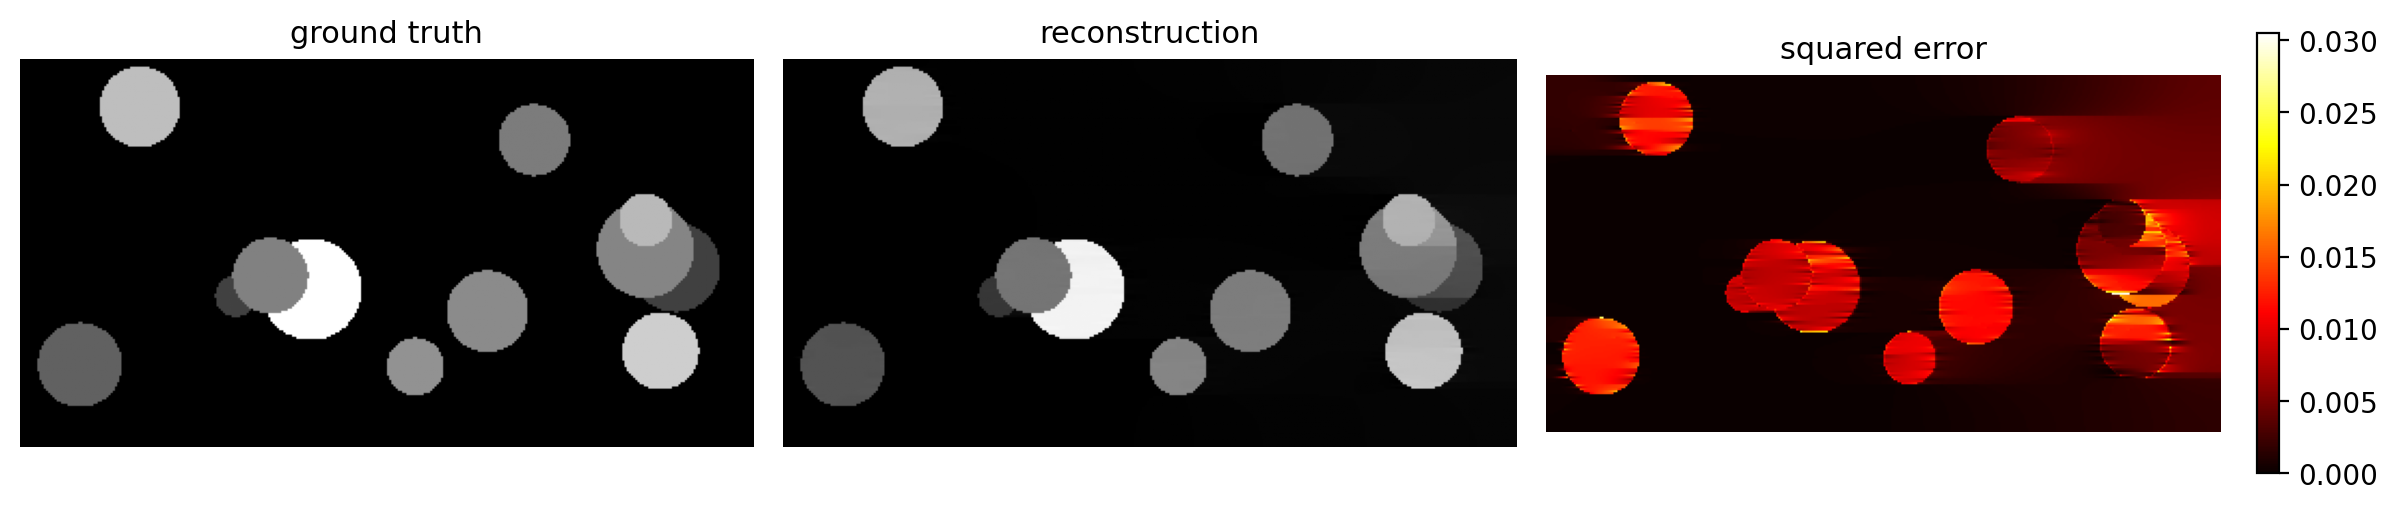
\includegraphics[width=\linewidth,height=2.55cm,keepaspectratio]{figures/sar_synthetic/disks_v2e.png}\par
% source: Ch. 2 sec:ch2_sar_bridge and fig:ch2_sar_synthetic; one-pixel horizontal translation per view, v2e events, smoothed-TV penalty.
{\scriptsize Simulated events (v2e~\cite{hu2021v2e}); the camera window shifts $1$\,px per view. Left: scene. Center: shared-scene estimate (smoothed-TV penalty). Right: squared error.\par}
\raggedright\vspace{1mm}
\begin{columns}[c]
\column{.50\textwidth}
\small\textbf{Chapter 2:} each pixel has its own temporal profile.\par\smallskip
\textbf{Shared scene:} known motion $P$ maps one static scene $\theta$ into every view.
\column{.46\textwidth}
% source: Ch. 2 eq:ch2_sar_forward.
\[\underbrace{B_{\rm SAR}}_{\text{scene-to-event operator}}=(A\otimes I)\,P.\]
\end{columns}
% source detail: Ch. 2, sec:ch2\_sar\_bridge, eq:ch2\_sar\_forward, prop:ch2\_sar\_solvability, fig:ch2\_sar\_synthetic.
\src{\dref{Figure}{fig:ch2_sar_synthetic}, \dref{Eq.}{eq:ch2_sar_forward}, \dref{Proposition}{prop:ch2_sar_solvability}; joint ESAR work~\cite{antil2026esareventbasedsyntheticaperture}; synthetic aperture~\cite{vaish2006synthetic}.}
\talknote{Shared-scene bridge; about 60 seconds. One idea: one scene, many views.}{Chapter 2 reconstructs independent pixel histories. In the joint ESAR work, $\theta$ is one static scene, the row-normalized footprint projections $P_k$ encode known motion and map it into each view, and $A$ differences consecutive views. The figure: twelve disks seen through a window translating one pixel per view; error concentrates along rows through the disks, the weakly constrained direction for horizontal motion. Chapter 3 then makes the motion itself the unknown.}{If asked for the algebra (Proposition 2.4.1): $\ker B_{\rm SAR}=\{\theta:P_{k+1}\theta=P_k\theta\}$ contains constants because $P_k\mathbf1=\mathbf1$; under translation, fields constant along the motion are weakly constrained. With unsquared ridge $\lambda>0$, $(B^\top B+\lambda I)\widehat\theta=B^\top b$ has a unique solution and $\norm{\delta\theta}\le\norm{B_{\rm SAR}}\norm{\delta b}/\lambda$. The figure uses a smoothed-TV penalty with the constant offset removed; the ridge result is the quadratic version of the same model. Other invariant modes depend on $P$ and the trajectory. JIF in Chapter 4 applies the same shared-unknown idea to two cameras.}
\end{frame}

\section{Dense optical flow}
\begin{frame}{The aperture problem: what a local view reveals}
\small An \textbf{aperture} is a restricted observation window: a small view of an edge~\cite{marr1981directional}.
\vspace{2mm}
\begin{columns}[T]
\column{.49\textwidth}\centering
\textbf{Through the windows}\par
\ifdefined\DefenseNotes
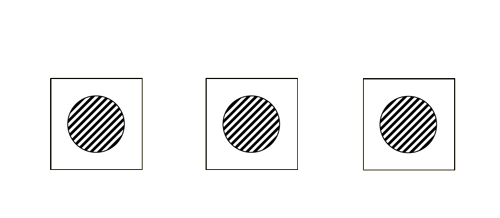
\includegraphics[width=\linewidth,height=2.65cm,keepaspectratio]{figures/aperture/masked.png}
\else
\ifdefined\DefensePresenter
\movie[loop]{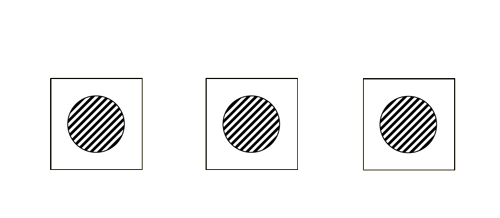
\includegraphics[width=\linewidth,height=2.3cm,keepaspectratio]{figures/aperture/masked.png}}{figures/aperture/app5-hide.mp4}
\else
\animategraphics[label=aperturemasked,width=\linewidth,height=2.3cm,keepaspectratio,poster=first,loop,controls={play,stop},buttonsize=2.5mm,buttonfg=0:0.498:0.514,method=widget,alttext={Masked stripes with ambiguous local motion}]{5}{figures/aperture/app5-hide/frame-}{0}{6}
\fi
\fi\par
{\footnotesize The visible stripe motions look the same.}\par\smallskip
\href{https://cdn.sinauer.com/wolfe4e/ch/08/act0802/app5-hide.gif}{\scriptsize\textcolor{teal}{Movie 5 source (GIF)}}
\column{.49\textwidth}\centering
\textbf{Reveal the full patterns}\par
\ifdefined\DefenseNotes
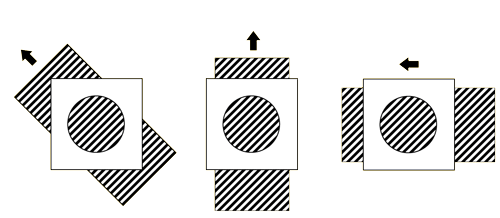
\includegraphics[width=\linewidth,height=2.65cm,keepaspectratio]{figures/aperture/revealed.png}
\else
\ifdefined\DefensePresenter
\movie[loop]{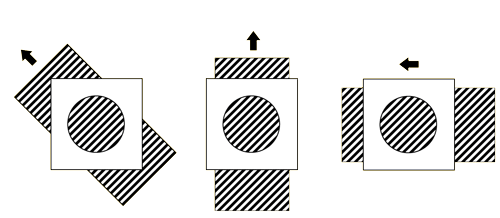
\includegraphics[width=\linewidth,height=2.3cm,keepaspectratio]{figures/aperture/revealed.png}}{figures/aperture/app6-show.mp4}
\else
\animategraphics[label=aperturerevealed,width=\linewidth,height=2.3cm,keepaspectratio,poster=first,loop,controls={play,stop},buttonsize=2.5mm,buttonfg=0:0.498:0.514,method=widget,alttext={Full stripe patterns with distinct translation directions}]{5}{figures/aperture/app6-show/frame-}{0}{6}
\fi
\fi\par
{\footnotesize The patterns translate in different directions.}\par\smallskip
\href{https://cdn.sinauer.com/wolfe4e/ch/08/act0802/app6-show.gif}{\scriptsize\textcolor{teal}{Movie 6 source (GIF)}}
\end{columns}
% source detail: Ch. 3, prop:time_surface and following aperture remark.
\vfill{\fontsize{6.5}{8}\selectfont\color{muted}Perceptual illustration: Wolfe et al., \emph{Sensation and Perception}, 4th ed., Sinauer \textcopyright\ 2015. \href{https://cdn.sinauer.com/wolfe4e/wa08.02.html\#Aperture}{\textcolor{teal}{Activity 8.2, Movies 5--6}}.\par Dissertation: \dref{Proposition}{prop:time_surface} and the following aperture discussion.\par}
\talknote{Define the aperture problem visually; about 90 seconds.}{Optical flow is apparent velocity in the image plane. An aperture simply means a restricted observation window. First look at the circular windows: the moving stripes look alike. Revealing the full patterns shows three different translation directions. A local straight edge tells us its speed perpendicular to the edge; motion along its tangent stays free. These publisher animations illustrate motion perception. They are conceptual demonstrations, rather than measured event-camera data.}{The two animations are embedded on this slide. Play the masked panel first using its forward-play control, then play the revealed panel; each loops at the original rate. First-frame posters preserve the visual comparison in static viewers and print. Use a PDF viewer with animation support and JavaScript enabled, as documented with the assets. Under steady illumination, different velocities with the same normal component produce the same local brightness changes and ideal events. Smoothness couples neighboring velocity estimates, while additional observed directions constrain the component left free by a single edge. Next, draw the same ambiguity for one edge and state the flow model in scene terms.}
\end{frame}

\begin{frame}{Motion introduces a new invisible direction}
\footnotesize
\vspace*{-3mm}
\begin{columns}[T]
\column{.47\textwidth}\centering
{\scriptsize\textbf{Image: one moving edge}}\par\smallskip
\begin{tikzpicture}[x=.45cm,y=.45cm,>=Latex]
\fill[soft] (0,0) rectangle (6,4);
\draw[ink,very thick] (2,0)--(2,4);
\draw[teal,very thick,->] (2,2)--(4.4,2) node[right,font=\scriptsize,align=left] {normal\\motion};
\draw[amber,very thick,->] (2,2)--(2,3.5) node[left,font=\scriptsize] {tangent};
\draw[muted,dashed] (4,0)--(4,4);
\end{tikzpicture}\par
{\scriptsize A straight edge reveals its normal speed.}
\column{.51\textwidth}\centering
{\scriptsize\textbf{Velocity: what the events allow}}\par\smallskip
\begin{tikzpicture}[x=.4cm,y=.4cm,>=Latex]
\draw[muted,->] (-.3,0)--(5.6,0) node[right,font=\scriptsize] {$v_x$};
\draw[muted,->] (0,-.3)--(0,4.4) node[left,font=\scriptsize] {$v_y$};
\draw[ink,very thick] (2.5,-.2)--(2.5,4.3) node[right,font=\scriptsize] {edge 1 constraint};
\draw[ink,very thick] (.6,3.9)--(4.2,.3) node[pos=.9,above right,font=\scriptsize] {edge 2 constraint};
\draw[ink,thick,->,shorten >=3.5pt] (0,0)--(2.5,2) node[pos=.45,above left,font=\scriptsize] {$\mathbf v$};
\draw[teal,very thick,->] (0,0)--(2.5,0);
\draw[amber,very thick,->,shorten >=3.5pt] (2.5,0)--(2.5,2);
\draw[ink,fill=white,thick] (2.5,2) circle (3.5pt);
\fill[ink] (2.5,2) circle (1.8pt);
\end{tikzpicture}\par
{\scriptsize Edge 1 fixes the {\color{teal}normal} part; edge 2, if it shares the motion, fixes the {\color{amber}tangent} part.}
\end{columns}
\vspace{0mm}
\vspace{1mm}
{\scriptsize\textbf{Flow model:} events give each edge's normal speed; neighbors moving alike supply the rest.\par
\textbf{Requirement (main theorem):} edges in two orientations somewhere, so their constraint lines cross.\par}
% source detail: Ch. 3, prop:time_surface and aperture remark (normal-speed constraint); thm:unified_wellposedness (integrated identifiability). Velocity-space intersection of constraints: Adelson and Movshon (1982).
\ifdefined\DefenseCommittee\vspace{-1mm}{\fontsize{6.5}{8}\selectfont\color{muted}Intersection of constraints [Adelson \& Movshon 1982]. Dissertation: \dref{Proposition}{prop:time_surface}; requirement in \dref{Theorem}{thm:unified_wellposedness}.\par}\fi
\talknote{Flow model in scene terms; about two minutes.}{A pixel fires when its log brightness changes by the threshold, so firing times trace an image edge. Left: normal motion in teal, tangent in amber. Right, velocity space, no positions: each line is every velocity one edge's events allow. Teal is the normal part edge 1 measures; amber is the tangent part it leaves free. If edge 2 shares the motion, the lines cross at $\mathbf v$, teal plus amber. Shared motion is an assumption: non-parallel lines always cross, so for edges moving differently the crossing is wrong for both. Requirement: two orientations somewhere.}{With exact coefficients and one shared velocity, the constant field is the unique minimizer at any $\alpha$ and separation. Example: edge 1 vertical moving right at $s$, edge 2 with normal $(1,1)/\sqrt2$ stationary; estimate $(s,-s)$ everywhere. Time-surface coefficient at an edge: rank one, proportional to $\mathbf n\mathbf n^\top$; two non-parallel normals give a positive-definite sum, the integrated condition. Slide 19: stripes give one orientation inside, the checkerboard two. Intersection of constraints: Adelson and Movshon.}
\end{frame}

\begin{frame}{Three representations, one quadratic variational problem}
Rename the flow data matrix $\B$ to distinguish it from temporal $\A$:
\[E_{\B,b}(\vct)=\frac12\int_\Omega\bigl(\vct^\top\B\vct-2b^\top\vct\bigr)
+\frac{\alpha^2}{2}\int_\Omega|\nabla\vct|^2.\]
\renewcommand{\arraystretch}{1.2}
\begin{tabular}{llll}\toprule Representation & $\B$ & $b$ & Edge measurement from\\\midrule
Time surface & $\nabla\mathcal T\nabla\mathcal T^\top$ & $\nabla\mathcal T$ & crossing times\\
Voxel projection & $\nabla a\nabla a^\top$ & $-a_s\nabla a$ & transported event activity\\
Structure tensor & $\widetilde{\mathbf J}$ & $-\mathbf j_t$ & gradients pooled over a window\\\bottomrule
\end{tabular}
\par\smallskip
{\footnotesize In scene terms: $\B$ records which motion directions the edges measure, and how strongly; $b$ carries the measured values; the $\alpha$ term asks neighbors to move alike.\par}
% source detail: Ch. 3, thm:unified\_wellposedness and its three corollaries.
\src{\dref{Theorem}{thm:unified_wellposedness} and its three corollaries; data-plus-smoothness form~\cite{horn1981determining}.}
\talknote{Unification; 60 seconds.}{The energies agree with the representation-specific residual energies up to an overall positive factor and a constant independent of flow. The common space is H\textasciicircum{}1(Omega; R\textasciicircum{}2), and the Dirichlet term couples neighboring velocities.}{The notation B here is A\_data in the dissertation, and alpha is alpha\_smooth. The change avoids using A for two different operators on consecutive chapters. The common analysis is about fixed coefficients. A good mathematical estimator can still encode a poor representation of physical motion. Scene terms: $\B$ records which motion directions the edges measure and how strongly; $b$ the measured values.}
\end{frame}

\begin{frame}{The main flow theorem: global information controls constants}
\begin{block}{Unified well-posedness theorem}
Let $\Omega\subset\R^2$ be bounded, connected, and Lipschitz; $\alpha>0$.
Assume
\[\B\in L^\infty,\quad \B=\B^\top\succeq0\text{ a.e.},\quad b\in L^2,\qquad
\setlength{\fboxsep}{1.5pt}\boxed{\int_\Omega\B(\mathbf x)\,d\mathbf x\succ0}.\]
Then $E_{\B,b}$ has a unique minimizer in $H^1(\Omega;\R^2)$.
\end{block}
\vspace{1mm}
The integrated matrix must identify \textbf{every constant velocity direction}.\par
\small In scene terms: edges in two or more orientations somewhere, so their constraint lines cross; neighbors supply the motion where $\B=0$.
% source detail: Ch. 3, thm:unified\_wellposedness, eq:integrated\_identifiability.
\src{\dref{Theorem}{thm:unified_wellposedness}, \dref{Eq.}{eq:integrated_identifiability}; classical quadratic-flow theory~\cite{weickert2001theoretical}.}
\talknote{Central theorem; 90 seconds.}{Classical quadratic optical flow already has well-posedness theory, including Weickert and Schn\"orr. The contribution here is one analysis for three event-derived coefficient constructions, with explicit identifiability and perturbation hypotheses. Read the hypotheses and interpret each. Connectedness makes the kernel of the gradient consist of global constants. The positive regularization coefficient controls spatial variation. Bounded data curvature and L2 forcing make the weak forms bounded. Positive definiteness of the integrated B controls constant fields that smoothness cannot see.}{B may vanish on open subsets while its integral remains positive definite. In these observation models the residual forcing b also vanishes there, and smoothness propagates information from observed regions. For time surfaces, no nonzero vector can be perpendicular to all measured gradients almost everywhere. The condition need not hold pointwise. Scene terms: edges in at least two orientations somewhere in the image. The one hypothesis the scene must supply; if it fails, a uniform slide along the null direction leaves the energy unchanged (Backup 35). It is checked on represented data, including smoothing artifacts at never-fired pixels. Accuracy rests on slide 16's shared-motion assumption (measured on slide 19).}
\end{frame}

\begin{frame}{Known-motion examples make the aperture problem visible}
\centering\small
\begin{tabular}{lccc}
 & Ground truth & Voxel & Structure tensor\\
\rotatebox{90}{Stripes}\! & 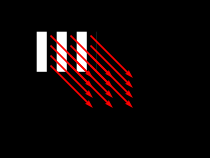
\includegraphics[width=2.75cm]{figures/ch3_quivers_consistent/v2e_stripes_f0022/crop/gt.png}&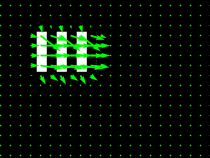
\includegraphics[width=2.75cm]{figures/ch3_quivers_consistent/v2e_stripes_f0022/crop/vox.png}&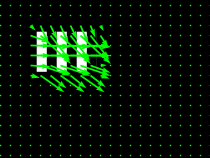
\includegraphics[width=2.75cm]{figures/ch3_quivers_consistent/v2e_stripes_f0022/crop/vox_struct.png}\\
\rotatebox{90}{Checker}\! & 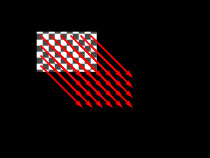
\includegraphics[width=2.75cm]{figures/ch3_quivers_consistent/v2e_checker_f0022/crop/gt.png}&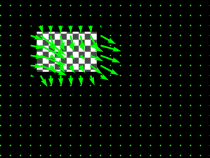
\includegraphics[width=2.75cm]{figures/ch3_quivers_consistent/v2e_checker_f0022/crop/vox.png}&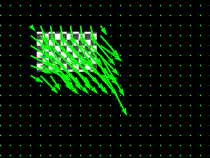
\includegraphics[width=2.75cm]{figures/ch3_quivers_consistent/v2e_checker_f0022/crop/vox_struct.png}\\
\end{tabular}
% source detail: Ch. 3, fig:ch3\_quiver\_v2e; v2e simulation, same window and arrow scale.
\src{\dref{Figure}{fig:ch3_quiver_v2e}; v2e~\cite{hu2021v2e} simulation, same window and arrow scale.}
\talknote{Visual evidence; 60 seconds.}{The object translates diagonally. Red arrows show the ground truth and green arrows the estimates, at the common scale retained from the dissertation's panels. Vertical stripe interiors provide mainly horizontal gradients. The checkerboard provides gradient information in both spatial directions. Object boundaries can supply additional information even in the stripe scene.}{These are selected illustrative windows, not a cross-dataset method ranking. The full figure also includes time surface and other variants; its reported TS AEE equals the zero-field baseline at the reported precision. The output does not diagnose which hypothesis or extraction step fails, so do not assign a cause.}
\end{frame}

\section{Stereo depth}
\begin{frame}{Stereo depth: competitive accuracy, most scored points}
\begin{columns}[c]
\column{.38\textwidth}\centering
\begin{tikzpicture}[x=.5cm,y=.36cm,>=Latex]
\coordinate (L) at (0,0);\coordinate (R) at (5,0);\coordinate (P) at (2,4);
\draw[ink,thick] (L)--(P)--(R);\fill[teal] (P) circle(2pt) node[above,font=\scriptsize] {scene point};
\draw[teal,thick] (-.6,1)--(1.2,1);\draw[teal,thick] (3.8,1)--(5.6,1);
\fill[ink] (L) circle(2pt) node[below,font=\scriptsize] {left};\fill[ink] (R) circle(2pt) node[below,font=\scriptsize] {right};
\draw[<->,amber] (0,-1.4)--(5,-1.4) node[midway,below,font=\scriptsize] {baseline $b_{\rm cam}$};
\draw[<->,muted] (5.9,0)--(5.9,4) node[midway,right,font=\scriptsize] {$Z$};
\end{tikzpicture}
\column{.58\textwidth}
\small
\[Z=\frac{f_{\rm cam}b_{\rm cam}}{d},\qquad d=x_L-x_R>0.\]
Each candidate $d$ pairs the two views, and one shared temporal profile is fitted to both. For fixed $d$ and frozen weights the inner solve is unique.
\end{columns}
\vspace{2mm}
\centering\footnotesize
\begin{tabular}{lrrrrrr}
\toprule & \multicolumn{4}{c}{Mean depth error (cm) $\downarrow$}&log RMSE&Scored\\
Method & Fl1&Fl2&Fl3&Fl4&$\times100\;\downarrow$&points (M)\\\midrule
% source: appendix_bodies/ch4_protocol.tex tab:unified_benchmark, wls row (mean error, log RMSE x100, #Pts).
\textbf{WLS (ours)}&73.83&\textbf{58.35}&70.33&59.24&\textbf{44.54}&\textbf{2.66}\\
% source: appendix_bodies/ch4_protocol.tex tab:unified_benchmark, Piatkowska row.
Piatkowska adaptation~\cite{piatkowska2017}&\textbf{67.96}&58.75&\textbf{68.88}&\textbf{54.63}&44.72&1.20\\\bottomrule
\end{tabular}\par\smallskip
% source: appendix_bodies/ch4_protocol.tex tab:metrics, per-method population; depth band [0.5,8] m; tab:unified_benchmark: 2.66M is the largest of the five methods.
{\scriptsize MVSEC indoor flying 1--4; each method scored on its own estimates in $[0.5,8]$\,m. Three more methods in the backup table.\par}
% source detail: Ch. 4, sec:solution, eq:depth\_conversion, thm:weighted\_spd; App., tab:unified\_benchmark, tab:metrics. Geometry is schematic.
\src{\dref{Section}{sec:solution}, \dref{Eq.}{eq:depth_conversion}, \dref{Theorem}{thm:weighted_spd}; \dref{Table}{tab:unified_benchmark}; MVSEC~\cite{MVSEC2018}. Geometry is schematic.}
\talknote{Stereo summary; about 3 minutes.}{Rectification places corresponding rays on the same image row; disparity is the horizontal shift and similar triangles give depth. At each candidate disparity, two softly coupled temporal profiles are solved; with frozen positive weights the Hessian is at least $\lambda_{\min}^2\mathbf I$, the Chapter 2 argument with one more nonnegative term. The benchmark uses the full WLS method: weight updates, cost aggregation, and candidate selection.}{WLS leads on Flying 2 and log RMSE; the Piatkowska adaptation leads on Flying 1, 3, and 4 by 5.9, 1.5, and 4.6 cm; WLS scores 2.66M points, the most of the five methods and 2.2 times Piatkowska's. Each method is scored on its own valid pixels, so read accuracy together with coverage. Correspondence questions go to the Chapter 4 backups.}
\end{frame}

\section{Contributions and next questions}
\begin{frame}{Research opportunities}
\small
\begin{columns}[T]
\column{.24\textwidth}
\begin{block}{Sensor modeling}
Measure the error terms of slide~9 on real sensors; the stability bounds turn them into estimate bounds.
\end{block}
\column{.24\textwidth}
\begin{block}{Learned weights}
Learn $\Lam$ in an outer problem [Antil--Di--Khatri 2020]; for $\Lam\succ0$, $\mathbf f^*(\Lam)$ is smooth.
\end{block}
\column{.24\textwidth}
\begin{block}{Shared scenes}
Find the motion-invariant modes of $B_{\rm SAR}$ for a trajectory (ESAR~\cite{antil2026esareventbasedsyntheticaperture}); apply to orbital streams.
\end{block}
\column{.24\textwidth}
\begin{block}{Edge hardware}
Update only pixels with events; measure time and power on a Raspberry Pi~5 and edge sensors.
\end{block}
\end{columns}
% source detail: Ch. 2, subsubsec:physical, thm:uniqueness, prop:ch2\_sar\_solvability; Ch. 3, eq:abstract\_stability; Ch. 5, Future Directions. External: Antil, Di, Khatri, Inverse Problems 36 (2020) 064001. Edge implementation: monocular_reconstruction/python/edge.
\src{\dref{Chapter}{ch:discussion_conclusion}, Future Directions; physical connection (\drefpage{subsubsec:physical}); \dref{Proposition}{prop:ch2_sar_solvability}. External paper cited above.}
\talknote{Future research; about 90 seconds.}{Sensor modeling: the identity on slide 9 names the error terms; measuring them on a real sensor gives the input the stability bounds need. The GMU Neuromorphic Imaging and Digital Twins Lab (AFOSR DURIP) makes those controlled acquisitions possible. Learned regularization: $\mathbf f^*(\Lam)=(\A^\top\A+\Lam^2)^{-1}\A^\top\mathbf y$ is rational and hence smooth in $\Lam$ on the positive orthant, which a bilevel analysis needs from its lower level.}{Shared scene: the ESAR null space contains constants and any other motion-invariant scene modes. Edge implementation: the streaming form updates each pixel in constant time; updating only pixels with events, and timing the method on a Raspberry Pi 5 with a power meter, are the next steps. Then go to the closing slide.}
\end{frame}

\begin{frame}{What the data constrain and what the models prove}
\footnotesize\renewcommand{\arraystretch}{1.05}
\begin{tabular}{>{\raggedright\arraybackslash}p{2.6cm}>{\raggedright\arraybackslash}p{4.4cm}>{\raggedright\arraybackslash}p{5.9cm}}\toprule
Problem & What the observations constrain & What the mathematical model establishes\\\midrule
Temporal reconstruction & Represented brightness increments & Unique regularized history for each fixed positive weight matrix, with perturbation bounds\\
Optical flow & Event-derived directional motion constraints & Unique $H^1$ minimizer under integrated identifiability\\
Stereo depth & Paired temporal event-feature observations & Unique frozen-weight inner solve; the disparity comes from a separate comparison of candidates\\\bottomrule
\end{tabular}
\takeaway{Under the stated hypotheses, regularization makes each estimator determinate; accuracy also depends on the representation.}
% source detail: Ch. 2 thm:uniqueness; Ch. 3 thm:unified\_wellposedness; Ch. 4 thm:weighted\_spd; Ch. 5, tab:contribution\_matrix.
\src{\dref{Theorem}{thm:uniqueness}, \dref{Theorem}{thm:unified_wellposedness}, \dref{Theorem}{thm:weighted_spd}; \dref{Table}{tab:contribution_matrix}.}
{\small\textcolor{teal}{\textbf{Which directions do the observations control, and which are selected by the model?}}\par\hfill Thank you.\par}
\talknote{Contributions and close; about 90 seconds.}{Read across each row: what the events constrain, then what the model proves. If asked about recomputed weights: Backup 65 (page 98) gives a local Lipschitz bound beyond the dissertation. The temporal null mode is selected by a penalty. Spatial smoothness and integrated directional data make the flow energy coercive. Stereo has a well-posed latent solve at each candidate; selecting the candidate is a separate decision.}{Close by returning to the common question, then stop for committee questions. Position the originality accurately: the functional-analytic tools are classical; the dissertation organizes event-derived models under explicit hypotheses and derives the coupling, conditioning, bias, and selection consequences. If asked about results beyond the table: contrast-maximization existence, graph convergence of the discrete flow, selection margins, and IRLS fixed-point and contraction results are in the backups and in Ch.\ 5, Table on the contribution matrix.}
\end{frame}
